\documentclass{article}
\usepackage[utf8]{inputenc}
\usepackage[english,russian]{babel}
\usepackage{multicol}
\usepackage{amsmath, amsfonts, amssymb, amsthm, mathtools}
\usepackage[a4paper, papersize={18cm, 23.5cm}]{geometry}
\usepackage{graphicx}
\usepackage{romannum}
% \newgeometry{top=1cm, bottom=1.8cm, left=0.8cm, right=1cm,marginal=30cm}
\geometry{bottom=0.8cm, right=1cm, left=0.8cm, top=1cm}
\usepackage{caption}
% Устанавливаем начальное значение счетчика для картинок
\setcounter{figure}{2 - 1} % Устанавливаем начальное значение счетчика для картинок, почему-то начинает на единицу больше
\captionsetup[figure]{labelfont=bf} % Выделяем "Рис." жирным
\captionsetup[table]{labelfont=bf}
\usepackage{scrextend} % уменьшение размера шрифта
\setlength\parindent{0} %parindent - Красная строка
\setlength{\columnsep}{1cm} 
\setlength{\parskip}{0pt}
\usepackage{xcolor}

\begin{document}
    % \documentclass{article}
% \usepackage[utf8x]{inputenc}
% \usepackage[english,russian]{babel}
% \usepackage{multicol}
% \usepackage{amsmath}
% \usepackage{geometry}
% \usepackage{graphicx}
% \thispagestyle{empty}
% \newgeometry{bottom=1cm, left=1.3cm, right=1.3cm, top=2cm}
% \begin{document}
\begin{center}
    \textbf{Университет ИТМО}\\
    \vspace{1em}
    Факультет Программной Инженерии и Компьютерной техники
    \vspace{9em}
    
    {\Large Информатика}\\[1em]
    {\Large Лабораторная работа \textnumero 6}\\[1em]
    {\Large \textbf{Работа с системой компьютерной вёрстки \TeX}}\\[1em]
    Вариант: $1 * 10 + 16 =$ \textbf{26}
\end{center}

\vspace{6em}

\begin{flushright}
    Выполнил: \\
    Ткачев Денис Владимирович\\
    Группа: P3111 \\
    Преподаватель: \\
    Малышева Татьяна Алексеевна \\
\end{flushright}
\vspace{10em}
\vfill
\begin{center}
Санкт-Петербург\\
2024г.
\end{center}
\clearpage
% \end{document}
    % \documentclass{article}
% \usepackage[utf8]{inputenc}
% \usepackage[english,russian]{babel}
% \usepackage{multicol}
% \usepackage{amsmath, amsfonts, amssymb, amsthm, mathtools}
% \usepackage[a4paper, papersize={18cm, 23.5cm}]{geometry}
% \usepackage{graphicx}
% \usepackage{romannum}
% % \newgeometry{top=1cm, bottom=1.8cm, left=0.8cm, right=1cm,marginal=30cm}
% \geometry{bottom=0.8cm, right=1cm, left=0.8cm, top=1cm}
% \usepackage{caption}
% % Устанавливаем начальное значение счетчика для картинок
% \setcounter{figure}{2 - 1} % Устанавливаем начальное значение счетчика для картинок, почему-то начинает на единицу больше
% \captionsetup[figure]{labelfont=bf} % Выделяем "Рис." жирным
% \captionsetup[table]{labelfont=bf}
% \usepackage{scrextend} % уменьшение размера шрифта
% \setlength\parindent{0} %parindent - Красная строка
% \setlength{\columnsep}{1cm} 
% \setlength{\parskip}{0pt}
% \usepackage{xcolor}
% % \setlength{\baseline}{0pt} % расстояние между абзацами
%     % \pagestyle{fancy} % Стиль страницы с верхним и нижним колонтитулами
%     % \fancyhead{} % Очистить верхний колонтитул
%     % \fancyfoot{} % Очистить нижний колонтитул


% \begin{document}

\begin{multicols}{2}
орбиты, если энергия спутника изменится на $\Delta E$.\\
$$E = -\frac{\mu m}{2a};~~ E + \Delta E = -\frac{\mu m}
{2(a+\Delta a)},$$
\begin{flushright}  
    (6)  
\end{flushright}\\
отсюда\\
\[\frac{\Delta E}{E} = -\frac{1}{1 + \frac{a}{\Delta a}} \approx -\frac{\Delta a}{a}\]\\
или\\
\begin{center}
    \hfill $\Delta a = -\frac{a}{E} \Delta E = \frac{2a^2}{\mu m}\Delta E.$ \hfill (7)
\end{center}

\hspace{1.5em}Найдем еще связь между изменением скорости и изменением кинетической энергии
$$K + \Delta K = \frac{m(v + \Delta v)}^2{2}$$\\
и\\
\begin{center}
    \hfill $\frac{\Delta K}{K} \approx 2\frac{\Delta v}{v}.$ \hfill (8)
\end{center}

Отсюда\\
\begin{center}
    \hfill $\Delta v = \frac{v}{2}\frac{\Delta K}{K} = -\frac{v}{2K}~\Delta E,$ \hfill (9)
\end{center}

т. к. из соотношения (5)
\begin{center}
    \hfill $\Delta K = -\Delta E.$ \hfill (10)
\end{center}


Подставляя теперь значение $\Delta E = F_{\text{т}}v\Delta t$, получим\\
\begin{center}
   \hfill $\Delta v = -\frac{1}{m}F_\text{т}\Delta t.$ \hfill (11)
\end{center}

\hspace{1.5em}Отсюда, считая изменения $\Delta v$ и $\Delta t$ малыми, получим выражение для ускорения спутника.\\

\begin{center}
    \hfill $W = -\frac{1}{m}F_{\text{т}}.$ \hfill (12)
\end{center}
\columnbreak

\hspace{1.5em}Это уравнение на вид противоречит второму закону Ньютона (знак минум перед F). На самом деле никакого противоречия, конечно, нет. Вспомним, что сила F представляет собой лишь возмущение по сравнению с доминирующей силой $\frac{1}{r^2}$. Из формулы (10) видно, что если энергия спутника увеличилась из-за увеличения радиуса орбиты на $\Delta E$, то кинетическая энергия уменьшилась на $\Delta E$. При этом потенциальная энергия увеличилась на $2\Delta E$, это и дало увеличение полной энергии.

\hspace{1.5em}Заметьте, что все наши рассуждения совершенно не зависят от того, какая именно возмущающая сила действует на спутник.

\hspace{1.5em}Исследуя зависимость всех этих величин от знака $\Delta E$, можно составить таблицу 1. Из нее видно, что в результате возрастания орбитальной энергии спутника его период, потенциальная энергия и размеры орбиты растут, а линейная скорость уменьшается. Если же сила, действующая на спутник, уменьшает его энергию, то это вызовет сокращение размеров орбиты и увеличение скорости.

\begin{center}
    \textbf{\Romannum{4}. Торможение в атмосфере}
\end{center}
\hspace{1.5em}Рассмотрим, что происходит при торможении спутника в земной атмосфере. В этом случае возмущающая (тормозящая) сила направлена против движения, то есть $\Delta E$ всегда имеет отрицательный знак. В соответствии с таблицей 1 большая полуось и период обращения будут постепенно убывать, следовательно, средняя
\vfill
\end{multicols}
\begin{table}[h!]
\hfill {\textbf{Таблица 1}\vspace{0.2cm}}
\begin{tabular}{p{16em}|c|c|c}
    \hline
    \multicolumn{1}{c|}{Величина} & \begin{tabular}{c}Обозначе-\\ние \end{tabular} & \begin{tabular}{c}Если $\Delta E > 0$\\(ускоряющая сила)  \end{tabular}& \begin{tabular}{c}Если $\Delta E < 0$\\ (тормозящая сила) \end{tabular}\\
    \hline
    Радиус орбиты (большая полуось в случае движения по эллипсу) & \raisebox{-0.5cm}{a} & \raisebox{-0.5cm}{увеличивается} &\raisebox{-0.5cm}{уменьшается} \\ %raisebox - делает ниже строку
    Период обращения & T & увеличивается & уменьшается \\
    Кинетическая энергия & K & уменьшается & увеличивается \\
    Потенциальная энергия & U & увеличивается & уменьшается \\
    Линейная скорость & $\upsilon$ & уменьшается & увеличивается \\
    \hline
\end{tabular}
\end{table}
\vfill \hfill \textbf{17}


\setlength{\columnsep}{1cm} 
\setlength{\parskip}{0pt}

\begin{multicols}{2}

\setlength{\fboxrule}{0.5pt} % Устанавливаем толщину рамки
\setlength{\fboxsep}{8pt} % Устанавливаем отступ от рамки до изображения
        \fcolorbox{blue}{white}{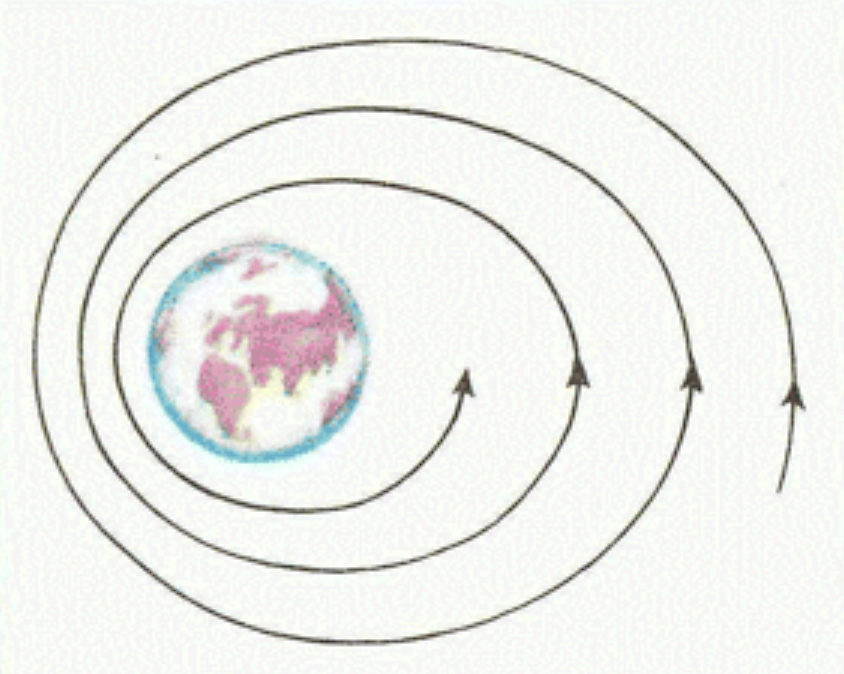
\includegraphics[scale=0.62]{квант 1.png}}
        \captionof{figure}{\textbf{Сжатие орбиты искусственного спутника при торможении в атмосфере.}}
        \label{fig:page}
        \vspace{1em}

        \vspace{10px}
        скорость должна расти. Теряемая потенциальаня энергия частично переходит в кинетическую, а остальная превращается в тепло. В перигее орбиты торможение максимально, потому что в этой точке скорость и атмосферная плотность принимают свои максимальные значения. В апогее же торможение будет минимальным. Поскольку в перигее спутник каждый раз получает отрицательный импульс, его орбита будет постепенно сжиматься, все сильнее приближаясь к круговой (рис. 2). Такое сжатие орбиты спутника под действием торможения в атмосфере неизбежно для всех искусственных спутников Земли и обычно сопровождается постепенным ростом скорости. Форма траектории приближается к окружности.
\columnbreak 

онных передач и для географических исследований.
На самом деле распределение массы Земли неоднородно, а форма ее отличается от шарообразной поэтому внешнее гравитационное поле тела, которое обладает тремя осями симметрии, а в сечении экваториальной плоскостью имеет эллипс. (На основе данных, полученных при исследовании траекторий спутников, можно сказать, что разность длин большой и малой осей эллиптического экваториального сечения Земли составляет 130 м, причем конец большой полуоси лежит на $15^\circ$ западной долготы).\par
\hspace{1.5em} Давайте посмотрим, как происходит движение спутника во вращающейся системе отсчета, а именно в системе отсчета, связанной с Землей (рис. 3). Из соображений симметрии ясно, что когда спутник находится на продолжении одной из главных осей экваториального эллипса (в точках A или B) гравитационная сила \dots 
\end{multicols}
\vfill \hfill \textbf{18}
% \end{document}
\end{document}